\documentclass[tikz,border=2pt]{standalone}

\usetikzlibrary{positioning}

\begin{document}
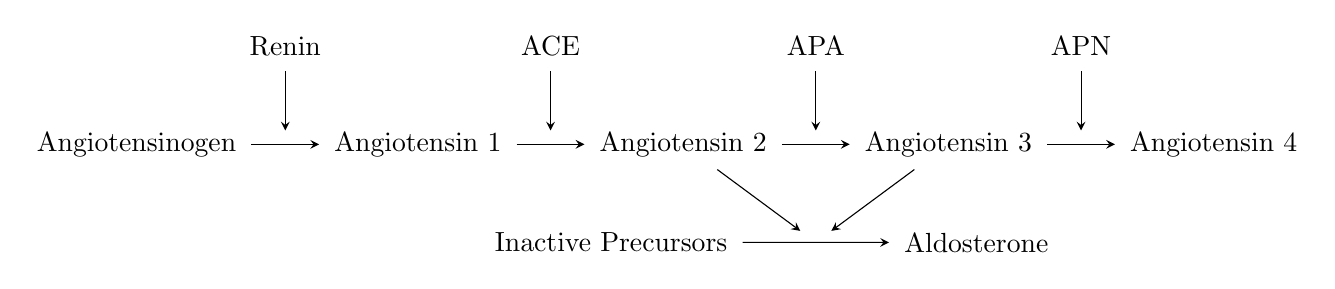
\begin{tikzpicture}
[shorten <=2pt,shorten >=2pt,>=stealth]
% nodes
\node [draw=none] (A) {Angiotensinogen};
\node [draw=none, right=of A] (B) {Angiotensin 1};
\node [draw=none, right=of B] (C) {Angiotensin 2};
\node [draw=none, right=of C] (D) {Angiotensin 3};
\node [draw=none, right=of D] (E) {Angiotensin 4};



% arrows 1
\draw [->] (A) -- coordinate (m1) (B);
\draw [->] (B) -- coordinate (m2) (C);
\draw [->] (C) -- coordinate (m3) (D);
\draw [->] (D) -- coordinate (m4) (E);

% nodes 2
\node [draw=none, above=of m1] (F) {Renin};
\node [draw=none, above=of m2] (G) {ACE};
\node [draw=none, above=of m3] (H) {APA};
\node [draw=none, above=of m4] (I) {APN};


% arrows 2
\draw [->, shorten >=5pt] (F) -- (m1);
\draw [->, shorten >=5pt] (G) -- (m2);
\draw [->, shorten >=5pt] (H) -- (m3);
\draw [->, shorten >=5pt] (I) -- (m4);

%nodes 3
\node [draw=none, below left=of m3] (J) {Inactive Precursors};
\node [draw=none, below right=of m3] (I) {Aldosterone};

% arrows 3
\draw [->] (J) -- coordinate (m5) (I);
\draw [->, shorten >=7pt] (C) -- (m5);
\draw [->, shorten >=7pt] (D) -- (m5);

\end{tikzpicture}

\end{document}